\documentclass{article}
\usepackage{v-equation}
\vgeometry

\begin{document}
\def\gdrive{https://drive.google.com/drive/folders/1PyqI8Hr2_Xaw06d3B0g0jQZGVms9bEs5?usp=share_link}

\vtitle[angular momentum]
\begin{center}
\begin{tikzpicture}
[thick]
\tzcoor*(0,  0)(O){$O$}[bl]
\tzcoor*($(O)!1!(45:2)$)(A)
	\tzline+[->](O)(45:2){$\vec{r}$}[mb]
	\tzline+[->](A)(0:2){$\vec{F}$}[r]
\end{tikzpicture}
\end{center}
\vspace*{\fill}
\addtolength{\jot}{3ex}
\begin{align*}
\vec{L} &= \left[ \vec{r} \vec{p}\right]\\
\dfrac{\d{\vec{L}}}{\d{t}} &= \left[\dfrac{\d{\vec{r}}}{\d{t}}, \vec{p} \right] + \left[ \vec{r}, \dfrac{\d{\vec{p}}}{\d{t}}\right]\\
\dfrac{\d{\vec{L}}}{\d{t}} &= 0 + \left[ \vec{r}, \dfrac{\d{\vec{p}}}{\d{t}}\right]\\
\vec{\tau} &= \left[ \vec{r}, \vec{F}\right]
\end{align*}
\vspace*{\fill}
\pagebreak

\vspace*{\fill}
\begin{center}
	\fbox{\qrcode[height=2cm]{\gdrive}}
\end{center}
\vspace*{\fill}
\end{document}
